
\section{Linearizzazione dei sistemi}
In mancanza della condizione di tempo invarianza può variare l'analisi del
sistema, verranno analizzati sistemi con discontinuità ma non sistemi che
variano con continuità nel tempo i loro parametri.

I sistemi non lineari sono composti da variabili e da parametri, i parametri
non sono mai forniti con un'accuratezza infinita, di conseguenza anche i
risultati in uscita avranno una certa incertezza.

Si suppone di modellare un sistema monodimensionale non lineare avendo fissato
una $\overline{u}(t)$ e si vuole mostrare l'andamento di $\dot x$ in funzione
di $x$, ricercando i vari punti di equilibrio.

%Curva di lavoro totale
\begin{figure}[h]
 \centering
 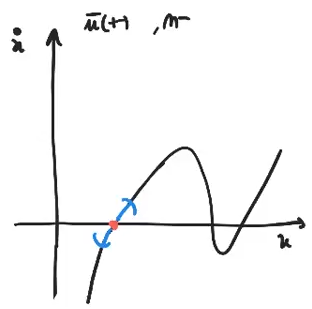
\includegraphics[width=\picwid]{curva_non_lineare.png}
 % curva_non_lineare.png: 312x309 px, 96dpi, 8.25x8.17 cm, bb=0 0 234 232
 \label{Fig.:curva_non_lineare}
\end{figure}

Si suppone che il sistema si trovi nel punto di lavoro $A$ indicato sul
grafico, nella realtà si troverà nell'intorno di quel punto oscillando in un
certo intervallo in funzione dei disturbi interni ed esterni al sistema.

Si suppone di ingrandire la curva nell'intorno del punto di lavoro

% Immagine ingrandita
\begin{figure}[h]
 \centering
 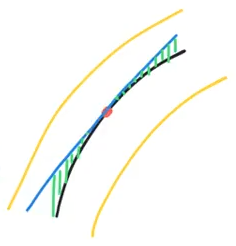
\includegraphics[width=\picwid]{curva_non_lineare_ingrandita.png}
 \label{Fig.:curva_non_lineare_ingrandita}
\end{figure}
Si considera una retta tangente alla curva nel punto di equilibrio, una retta è
sinonimo di un modello lineare, l'errore aggiuntivo commesso può ritenersi
trascurabile se minore dell'accuratezza fornita dal modello sesso.

Il vantaggio ottenuto da tale approssimazione è la possibilità di risolvere
analiticamente un sistema lineare piuttosto che cercare un teorema in grado di
risolvere quel particolare sistema non lineare.

Se si sposta di molto il punto di lavoro del sistema è necessario ricalcolare
la linearizzazione del sistema, non potendo più utilizzare la retta precedente.
Si ottiene ancora una buona approssimazione.

Ha senso linearizzare solo i punti di equilibrio, altrimenti il sistema non si
troverebbe nell'intorno di un punto, si potrebbe estendere il concetto anche a
punti di equilibrio dinamici.

$$\left\{
\begin{aligned}
\dot{x} &= f(x,u) \\
y &= g(x,u)
\end{aligned}\right.$$
Si ipotizza che le funzioni $f$ e $g$ siano sufficientemente regolari, ossia
che esista almeno il differenziale primo.

Si suppone inoltre che il sistema sottoposto ad un ingresso costante
$\overline{u}$ si trovi in un punto di equilibrio $\overline{x}$ a cui
corrisponde un'uscita di equilibrio $\overline{y}$, ossia
$$
(\overline{u},\overline{x},\overline{y}) \ \text{punto di equilibrio}
$$

Si applica la seguente posizione
$$
x(t) = \overline{x} + \delta x(t)
$$
dove $\delta x(t)$ è l'errore della traiettoria rispetto al punto di lavoro,
ovvero lo spessore definito prima nell'intorno del punto.

Analogamente per l'ingresso $u(t)$
$$
u(t) = \overline{u} + \delta u(t)
$$
Gli ingressi si suddividono in \textit{manipolabili} e \textit{non
manipolabili} dunque
anche gli ingressi sono affetti da errore e rumore,  è necessario tenere conto
di questi errori mediante
$$
y(t) = \overline{y}+\delta y(t)
$$

Tutte le precedenti equazioni sono vettoriali.

Derivando l'equazione dello stato
$$
\dot{x} = \dot{\overline{x}} + \dot{\delta x} = \dot{\delta x}
$$
quindi la variazione dello stato coincide con la variazione locale. Si può
sviluppare in serie di Taylor nel punto di equilibrio
\begin{equation}
\dot{\delta x} = \cancel{f(\overline{x},\overline{u})} + \left.\frac{\partial
f}{\partial x}\right|_{\text{eq}}\delta x + \left.\frac{\partial f}{\partial
u}\right|_{\text{eq}}\delta u + o(\delta x, \delta u)
\label{eq.:linearizzazione_sistema}
\end{equation}
La funzione di transizione valutata su un punto di equilibrio è nulla per
definizione di punto di equilibrio, il termine $\frac{\partial f}{\partial x}$
è una matrice Jacobiana con numero di righe pari al numero di righe della $f$
dunque $n$ ed un numero di colonne pari al numero di elementi della $x$, ancora
$n$ quindi è una matrice $n\times n$, la matrice verrà chiamata $A$.

Il termine $\frac{\partial f}{\partial u}$ ha invece $n$ righe ed $m$ colonne
dove $m$ è il numero di ingressi, verrà chiamata $B$.

Si riscrive la \ref{eq.:linearizzazione_sistema} trascurando l'o-piccolo si
ottiene

$$\begin{aligned}
\dot x &= \dot{\delta x} = A\delta x + B \delta u
\end{aligned}$$
quella ottenuta è proprio l'equazione di un sistema dinamico lineare con
variabile di stato pari a $\delta x$ ed ingresso pari a $\delta u$

La variazione dell'uscita invece sarà
$$\begin{aligned}
y &= \overline{y} + \delta y = g(\overline{x},\overline{u}) +
\left.\frac{\partial
g}{\partial x}\right|_{\text{eq}}\delta x + \left.\frac{\partial g}{\partial
u}\right|_{\text{eq}}\delta u + o(\delta x, \delta u) \\
\delta g &\simeq C\delta x + D \delta u
\end{aligned}$$
Anche la variazione dell'uscita è lineare con la variazione dello stato e
dell'ingresso.

Dopo aver risolto il sistema delle variazioni si somma con il sistema dei
punti di equilibrio e si ottiene la risoluzione dell'intero sistema.

In molti casi la coppia $(0,0)$ è un punto di equilibrio, in questo specifico
caso è sufficiente calcolare solo le variazioni, dato che andrebbero poi
sommate con un valore nullo di ingresso ed equilibrio.

\subsection{Linearizzazione del sistema di un pendolo}
Si riprende l'esempio analizzato alla sezione \ref{sec.:equilibrio_del_pendolo}
$$\left\{\begin{aligned}
\dot x_1 &= x_2\\
\dot x_2 &= - \frac{g}{l}\sin{x_1} + \frac{1}{mL}u \\
y &= x_1
\end{aligned}\right.$$

Va dunque calcolata la matrice $A$
$$ A =
\left.\frac{\partial f }{\partial x}\right|_{\text{eq}} = \begin{pmatrix}
 \left.\frac{\partial f_1}{\partial x_1}\right|_{\text{eq}}
 & \left.\frac{\partial f_1}{\partial x_2}\right|_{\text{eq}} \\
 \left.\frac{\partial f_2}{\partial x_1}\right|_{\text{eq}}
 & \left.\frac{\partial f_2}{\partial x_2}\right|_{\text{eq}}
\end{pmatrix} =
\begin{pmatrix}
 0 & 1\\
 -\frac{g}{L}\cos(\overline{x}_1) & 0
\end{pmatrix} $$

Si ripete il procedimento rispetto all'ingresso e si calcola la matrice $B$
$$
B = \left.\frac{\partial f }{\partial u}\right|_{\text{eq}} =
\begin{pmatrix}
 \left.\frac{\partial f_1}{\partial u}\right|_{\text{eq}} \\
 \left.\frac{\partial f_2}{\partial u}\right|_{\text{eq}}
\end{pmatrix} =
\begin{pmatrix}
0 \\
\frac{1}{mL}
\end{pmatrix}
$$
La seconda matrice è costante e non dipende dai punti di equilibrio.

Si esegue la stessa operazione per l'equazione delle uscite
$$
C = \left.\frac{\partial g}{\partial x}\right|_{\text{eq}} =
\begin{pmatrix}
 \left.\frac{\partial g}{\partial x_1}\right|_{\text{eq}}  &
 \left.\frac{\partial g}{\partial x_2}\right|_{\text{eq}}
\end{pmatrix} =
\begin{pmatrix}
 1 & 0
\end{pmatrix}
$$

Infine dato che il sistema è strettamente proprio non è necessario calcolare la
matrice $D$ dato che sarà sicuramente nulla, se ne riporta in ogni caso la
definizione
$$
D = \left.\frac{\partial g}{\partial u}\right|_{\text{eq}} =
0
$$
L'unica matrice che varia al variare del punto di equilibrio è la prima.

Si calcolano le matrici $A'$ ed $A''$ nei due punti di equilibrio
$$
\overline{u} = 0 \left\langle
\begin{aligned}
 \\
 \overline{x'} &= \begin{pmatrix}
                  0 \\ 0
                 \end{pmatrix} \Rightarrow
                 A' = \left.\frac{\partial f}{\partial x}
                            \right|_{\begin{aligned}
                                      x &= \overline{x'}\\
                                      u &= 0
                                     \end{aligned}} =
                                     \begin{pmatrix}
                                      0 & 1 \\
                                      -\frac{g}{L} & 0
                                     \end{pmatrix}
\\
 \overline{x''} &= \begin{pmatrix}
                   \pi \\ 0
                  \end{pmatrix} \Rightarrow
                 A'' = \left.\frac{\partial f}{\partial x}
                            \right|_{\begin{aligned}
                                      x &= \overline{x'}\\
                                      u &= 0
                                     \end{aligned}} =
                                     \begin{pmatrix}
                                      0 & 1 \\
                                      \frac{g}{L} & 0
                                     \end{pmatrix}
\end{aligned} \right.
$$

Al variare di un solo segno si vedrà come il sistema si comporterà in modi
completamente differenti, si studierà ossia la \textit{stabilità} del sistema.

\section{Richiami di geometria}
\subsection{Endomorfismo}
Si consideri un'applicazione che trasforma i vettori dello spazio
$\mathfrak{X}$ in altri vettori dello stesso spazio vettoriale.
Funzioni di questo tipo possono essere rappresentate da matrici $n\times n$
$$
x' = Ax\quad A\in\mathbb{R}^{n\times n}
$$
L'applicazione $A$ trasforma rette passanti per l'origine in altre rette
passanti per l'origine.
\begin{figure}[h]
 \centering
 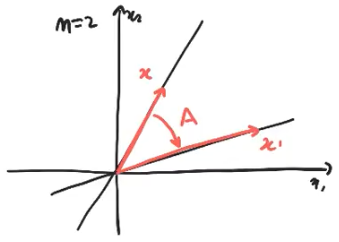
\includegraphics[width=\picwid]{endomorfismo_rette.png}
 % endomorfismo_rette.png: 339x242 px, 96dpi, 8.97x6.40 cm, bb=0 0 254 181
 \label{Fig.:endomorfismo_rette}
\end{figure}

\subsection{Trasformazione di similitudine}
Sia $x\in X^n$ e sia la matrice $T \in \mathbb{R}^{n\times n}$ non singolare
ossia con determinante diverso da zero e invertibile.

Se si hanno $n$ vettori indipendenti tra loro, possono essere considerati come
una \textit{base} per uno spazio vettoriale, si può dunque esprimere il vettore
$x$ nella base data da $T$
$$
x = T \tilde{x}
$$
Dato che $T$ è invertibile
$\tilde{x} = T^{-1}x$

Si consideri un vettore
\begin{equation}x' = Ax\label{eq.:endomorfismo}\end{equation}
dove $A$ è un endomorfismo. Se si vuole
rappresentare il vettore $x'$ in funzione della nuova base allora
$$
T\tilde{x}' = Ax = AT\tilde{x}
$$
Si moltiplica per l'inversa di $T$
$$
\tilde{x}' = T^{-1}AT \tilde{x}
$$
Quindi si è riscritta la relazione \ref{eq.:endomorfismo} ma nella nuova base,
ciò implica che la trasformazione $A$ è la stessa ma è avvenuta nel nuovo
sistema di riferimento.

Si può definire
$$
T^{-1}A T = \tilde{A}
$$
dove $\tilde{A}$ è una matrice \textit{simile} alla matrice $A$, la relazione
di similitudine è una condizione di uguaglianza, deve verificare tre proprietà:
\begin{itemize}
 \item Riflessiva:

    Se $A=\tilde{A}$ la trasformazione $T$ deve necessariamente essere la
matrice identità $T=I$
 \item Simmetria:

 Se $A=\tilde{A} \Rightarrow \tilde{A}=A$

 Si moltiplica il primo termine a destra per $T$ e a sinistra per $T^{-1}$
 \item Transitiva:

 Se $A=\tilde{A},\ \tilde{A}=\tilde{\tilde{A}} \Rightarrow A =
\tilde{\tilde{A}}$
\end{itemize}

Si consideri lo spazio delle matrici $\{A\in\mathbb{R}^{n\times n}\}$,
si può dividere in classi di equivalenza tra loro disgiunte, si possono
raggruppare tutte le matrici che appartengono alla stessa classe di
similitudine.

\subsection{Autospazi invarianti monodimensionali}
Si consideri un certo endomorfismo $A$ definito nello spazio $X^n$, esso
trasforma come già accennato, rette passanti per l'origine in rette passanti
per l'origine.

Esistono direzioni ``speciali'' per le quali, applicata $A$, si ottiene un
altro vettore che giace sul vettore di partenza, al limite cambiando in modulo.

La retta $Ax$ deve essere proporzionale per un fattore $\lambda$ ad $x$
\begin{align}
Ax &= \lambda x\\
(A-\lambda I)x &= \underline{0}
\label{eq.:autovalori}\end{align}
Quello appena ottenuto è un sistema algebrico \textit{omogeneo} di $n$
equazioni in $n$ incognite.
Dal teorema di Rouché-Capelli, ammetterà una soluzione non banale solo se la
matrice $(A-\lambda I)$ è singolare, ossia il suo determinante è nullo.
Il determinante della matrice produce un polinomio, nell'incognita $\lambda$ di
ordine $n$ detto anche \textit{polinomio caratteristico}
della matrice $A$.
(Il sistema omogeneo ammette il cambio di segno)
$$
\text{det}(\lambda I -A) = p(\lambda) = \lambda^n + \alpha_{n-1}\lambda^{n-1} +
\alpha_{n-2}\lambda^{n-2} + \dots + \alpha_0 = 0
$$
Si ricaveranno tutti i valori di $\lambda$ per i quali la matrice
$(A-\lambda I)$ è singolare.
Dal teorema fondamentale dell'algebra posso trovare $n$ soluzioni,
$\lambda_1,\dots,\lambda_n $ prendono il nome di \textbf{autovalori} della
matrice $A$.
Se la matrice $A$ è reale, i coefficienti sono tutti reali, un polinomio a
coefficienti reali può ammettere radici reali o complesse e coniugate.

Alcuni autovalori possono avere una molteplicità algebrica $m_{a}$ maggiore di
uno, ossia possono essere più volte soluzione del polinomio.
Ad esempio il polinomio
$$
(\lambda-1)^{3} = 0
$$
ammette come soluzione $\lambda =1$ con molteplicità algebrica $m_a = 3$.
Se gli autovalori sono tutti distinti fra loro, ossia  avranno tutti
molteplicità unitaria, la matrice $A$ si dirà di \textit{semplice struttura}.

Per ricavare le direzioni invarianti vanno trovati gli \textbf{autovettori},
vettori che giacciono nelle direzioni invarianti.
Se si sostituisce nella \ref{eq.:autovalori} il generico $\lambda_i$
\begin{equation}
(\lambda_i I -A)u_i = 0
\label{eq.:autovalori_sostituiti}
\end{equation}
Il vettore $u_i$ non nullo deve per costruzione giacere sulla direzione
invariante.
Se un autovalore $\lambda_i$ ha molteplicità $1$, la matrice
\ref{eq.:autovalori_sostituiti} ``perde  di rango'' una sola volta, quindi di
$n$ equazioni saranno $n-1$ indipendenti, con un solo grado di libertà, ossia
lo spazio vettoriale, soluzione del sistema sarà una retta, quindi un solo
autovettore.
Se la molteplicità dell'autovalore fosse $2$ allora anche lo spazio delle
soluzioni potrebbe essere di ordine $2$, dunque un piano o equivalentemente una
coppia di vettori.

La dimensione dell'autospazio invariante prende il nome di \textit{molteplicità
geometrica} dell'autovalore $m_{gi}$.

$$
m_{gi} = n - \rho(\lambda_i I -A)
$$

Non è possibile trovare un numero di autovettori maggiore della molteplicità
algebrica del relativo autovalore.
$$
1\leq m_{gi} \leq m_{ai}
$$
